\documentclass[14pt]{extreport}

\usepackage[utf8]{inputenc}
\usepackage[italian,english]{babel}
\usepackage{graphicx}
\usepackage{cite}
\usepackage{amsmath}
\usepackage[table,xcdraw]{xcolor}
\usepackage[italian]{minitoc}% per gli accenti
\usepackage{fancybox}
\usepackage{verbatim}
\usepackage{url}
\usepackage{color}
\usepackage{listings}
\usepackage{makeidx}
\usepackage{comment}
\usepackage{hyperref}
\usepackage{mathabx}
\usepackage{titlesec}

%cartella in cui sono contenute le immagini
\graphicspath{ {./Figure/} }


\titleformat{\chapter}{\normalfont\huge}{\textbf\thechapter.}{20pt}{\huge\textbf}

%inizio documento
\begin{document}
\selectlanguage{italian}

%inizio copertina
\begin{titlepage}
\begin{center}
	\begin{figure}
    	
\includegraphics[width=2.5cm, height=2.5cm]{unisa.png}
    	\centering
    \end{figure}
	{\Large Università degli Studi di Salerno}\\[0.2truecm]
	{\large Dipartimento di Informatica\\Corso di Laurea Triennale in Informatica}\\
	\hrulefill
	\vfill
	{\large Tecnologie Software per il WEB}\\[0.2truecm]
    {\large Project Proposal}\\[0.2truecm]
	%{\Large Informatica}\\
	\vfill\vfill
	{\LARGE {\bf CardHaven}}
	
	\vfill\vfill
	
	
	\ \ \ \ \ \ \ {\bf Docente} \hfill {\bf Studenti}\ \hfill  {\bf Matricola}\  \\
	Prof.  Simone Romano \hfill Squitieri Andrea \hfill 0512119008 \\
    \ \ \ \ \ \ \ \hfill \hfill \hfill Stefanile Andrea \hfill 0512119557 \\
    \ \ \ \ \ \ \ \ \ \ \ \ \ \ \ \ \ \ \ \ \ \ \hfill \hfill \hfill \hfill \hfill \hfill \hfill \hfill \hfill \hfill \hfill Tozza Gennaro Carmine \hfill 0512120382 \\
	\vfill
	\hrulefill 
	\begin{center} Anno Accademico 2024-2025 \end{center}
	
\end{center}
\end{titlepage}
%fine copertina

% -----------------------------------------
\tableofcontents

\chapter{Obiettivo del progetto}
\textbf{CardHaven} si configura come una piattaforma e-commerce specializzata nella vendita diretta di 
carte collezionabili e prodotti correlati. \\ Si rivolge a giocatori e collezionisti di 
vari giochi di carte (come Magic: The Gathering, Pokémon, Yu-Gi-Oh!, One Piece TCG, etc.), 
offrendo loro un punto di riferimento unico per i loro acquisti.\\\\
\noindent
L'obiettivo è fornire un catalogo ampio e costantemente aggiornato che comprenda non solo carte singole,
 bustine e box sigillati, ma anche una vasta gamma di accessori: bustine protettive 
 (sleeves), porta-mazzi (deck box), tappetini da gioco (playmat), dadi, segnalini e altri gadget a tema.\\\\
\noindent
Il sito mira a soddisfare il bisogno di reperire facilmente sia le ultime novità che articoli più datati, 
facilitando la ricerca e l'acquisto. \\ Intendiamo inoltre creare una community attiva permettendo agli 
utenti di condividere le proprie opinioni sui prodotti tramite recensioni.\\\\
\noindent
Per garantire accessibilità e usabilità, CardHaven sarà sviluppato con un design responsive, 
ottimizzato per la visualizzazione su computer desktop, tablet e smartphone.

% -----------------------------------------

\chapter{Analisi dei competitor}
\section{Federic Store}\footnote{\url{https://federicstore.it}}
Questo negozio online si concentra principalmente sul gioco di carte Pokémon, affiancando l'offerta con prodotti legati ad altri TCG e a specifici content creator. Dispone anche di un'applicazione mobile.

\begin{figure}[h!] 
    \centering
    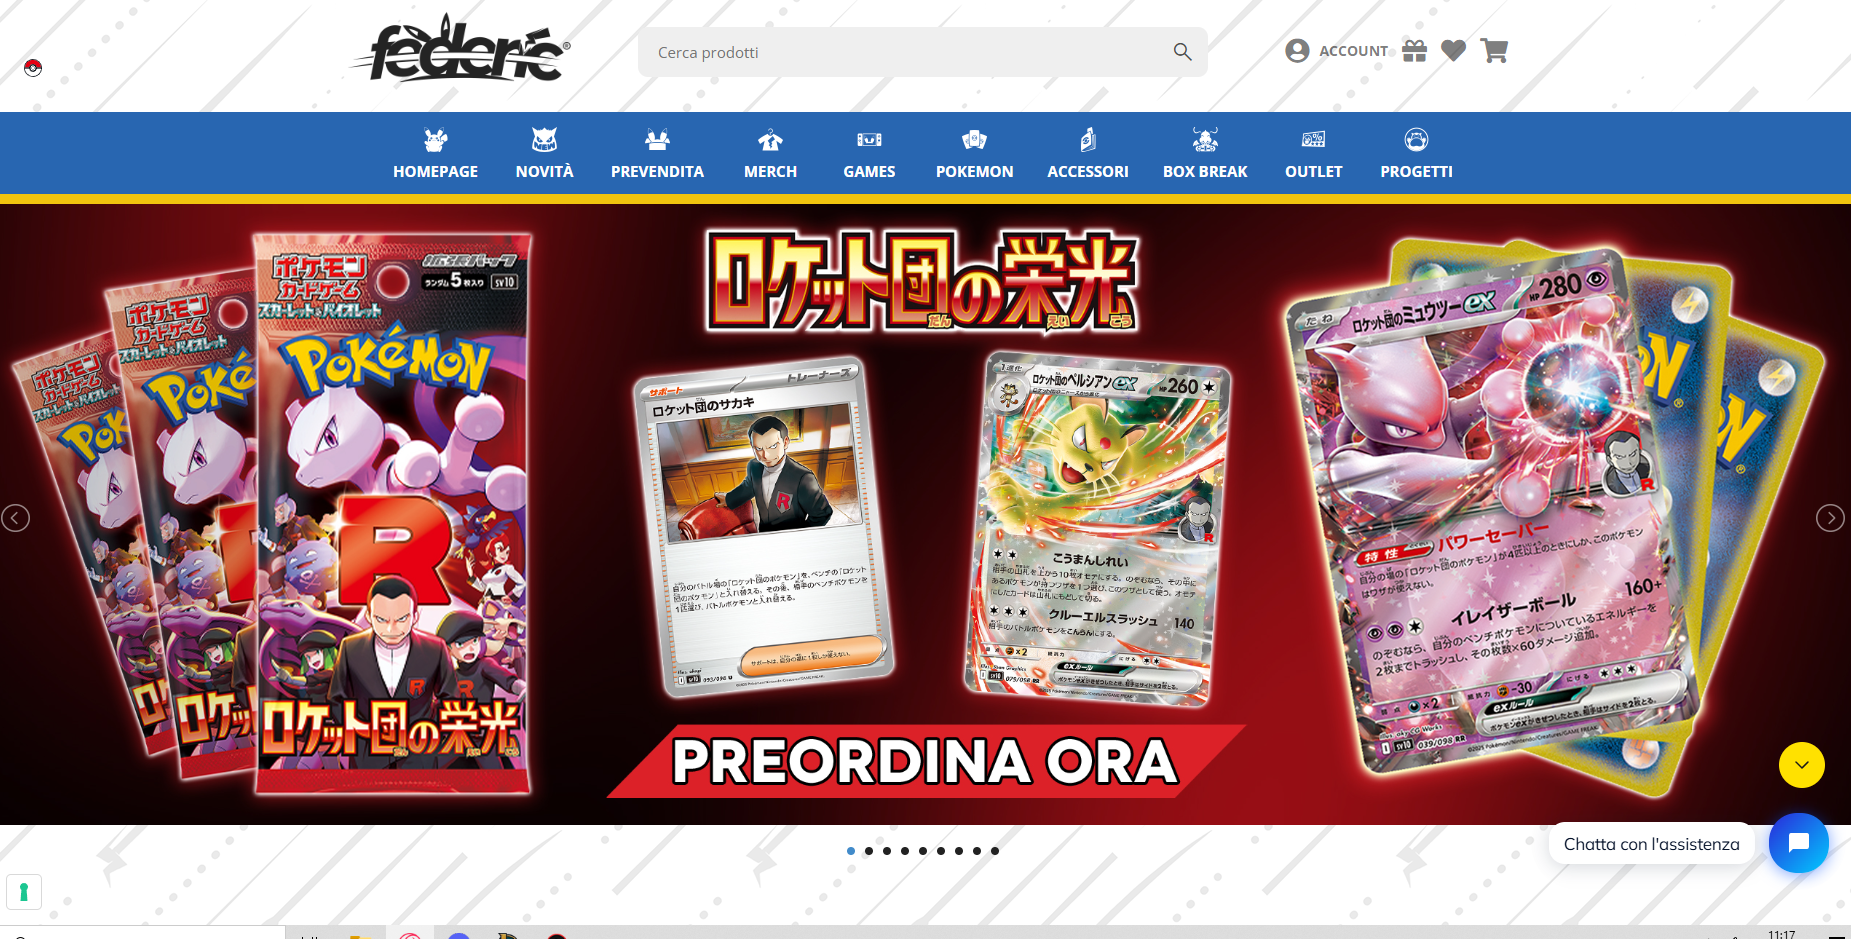
\includegraphics[width=0.8\textwidth]{federic-store.png}
    \caption{Homepage di Federic Store.}
\end{figure}

\begin{itemize}
    \item \textbf{Offerta Prodotti:} Il catalogo include carte singole Pokémon (con un filtro dedicato alla nazionalità delle carte), prodotti sigillati, accessori e merchandising a tema. Presenta anche articoli di altri giochi (es. One Piece) e prodotti esclusivi legati a collaborazioni.
    \item \textbf{Interfaccia e Navigazione:} Il sito web presenta una struttura orientata alla vendita, con categorie dedicate ai diversi tipi di prodotto (Pokémon, Altri Giochi, Accessori). Offre sezioni per novità, prevendite e sconti.
    \item \textbf{Funzionalità Principali:} Dispone di funzionalità standard di e-commerce come catalogo prodotti con filtri, carrello, gestione account utente. Offre diverse opzioni di pagamento, inclusi sistemi rateali, e un servizio di assistenza clienti. Include una sezione news a tema Pokémon (Pokénews).
\end{itemize}

\section{CarteMagic}\footnote{\url{https://www.cartemagic.com}}
Si tratta di un e-commerce italiano con un forte focus su Magic: The Gathering, ma che estende la propria offerta a numerosi altri giochi di carte collezionabili e relativi accessori.

\begin{figure}[h!]
    \centering
    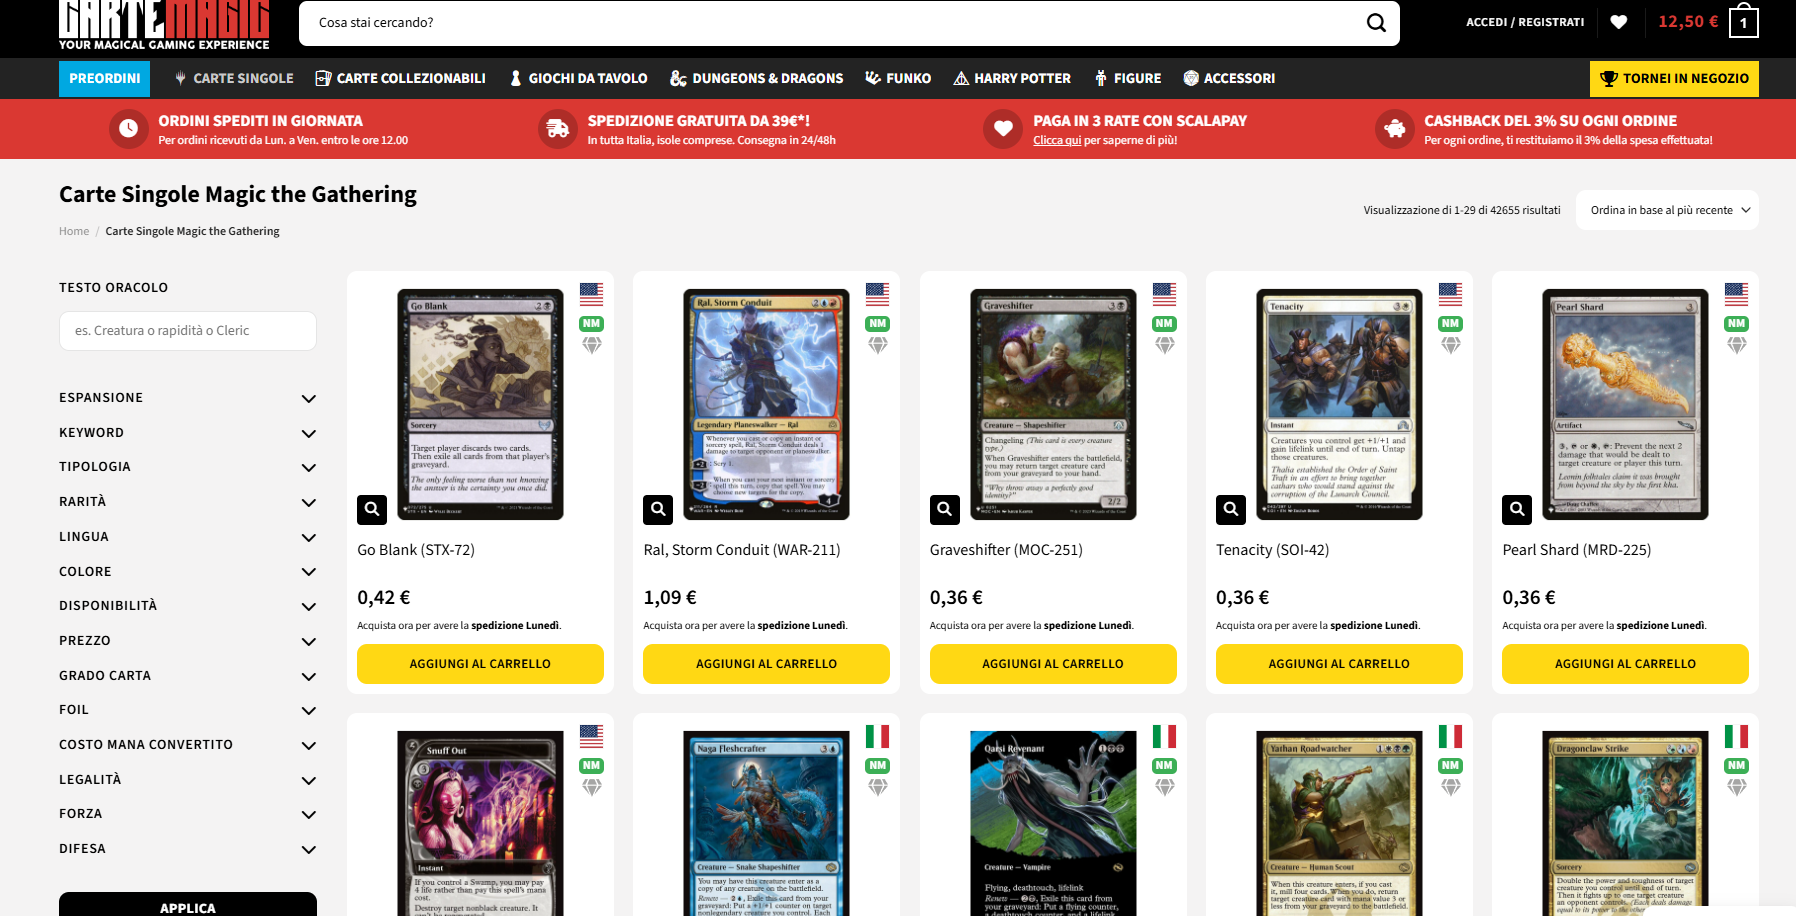
\includegraphics[width=0.8\textwidth]{carte-magic.png}
    \caption{Catalogo di CarteMagic.}
\end{figure}

\begin{itemize}
    \item \textbf{Offerta Prodotti:} Il catalogo è particolarmente fornito per Magic (carte singole, box, bustine, mazzi Commander) e include sezioni dedicate a Pokémon, One Piece, Yu-Gi-Oh!, Lorcana, Star Wars Unlimited e altri TCG popolari. Sono presenti anche accessori.
    \item \textbf{Interfaccia e Navigazione:} Il sito è organizzato principalmente per gioco, con sottocategorie per tipo di prodotto (sigillato, mazzi, accessori). Mette in evidenza alcune politiche commerciali come un programma di cashback e soglie per la spedizione gratuita.
    \item \textbf{Funzionalità Principali:} Offre strumenti di ricerca e filtro per navigare il catalogo, gestione del carrello e dell'account utente. Gestisce preordini con acconto e propone un programma di cashback sugli acquisti. Dichiara spedizioni rapide e opzioni di pagamento rateale.
\end{itemize}

\section{Cardgame-Club} \footnote{\url{https://cardgame-club.it}}
Questo store online si caratterizza per un catalogo estremamente ampio, che copre un numero molto elevato di giochi di carte collezionabili, giochi da tavolo, accessori di diverse marche e articoli di collezionismo.

\begin{figure}[h!]
    \centering
    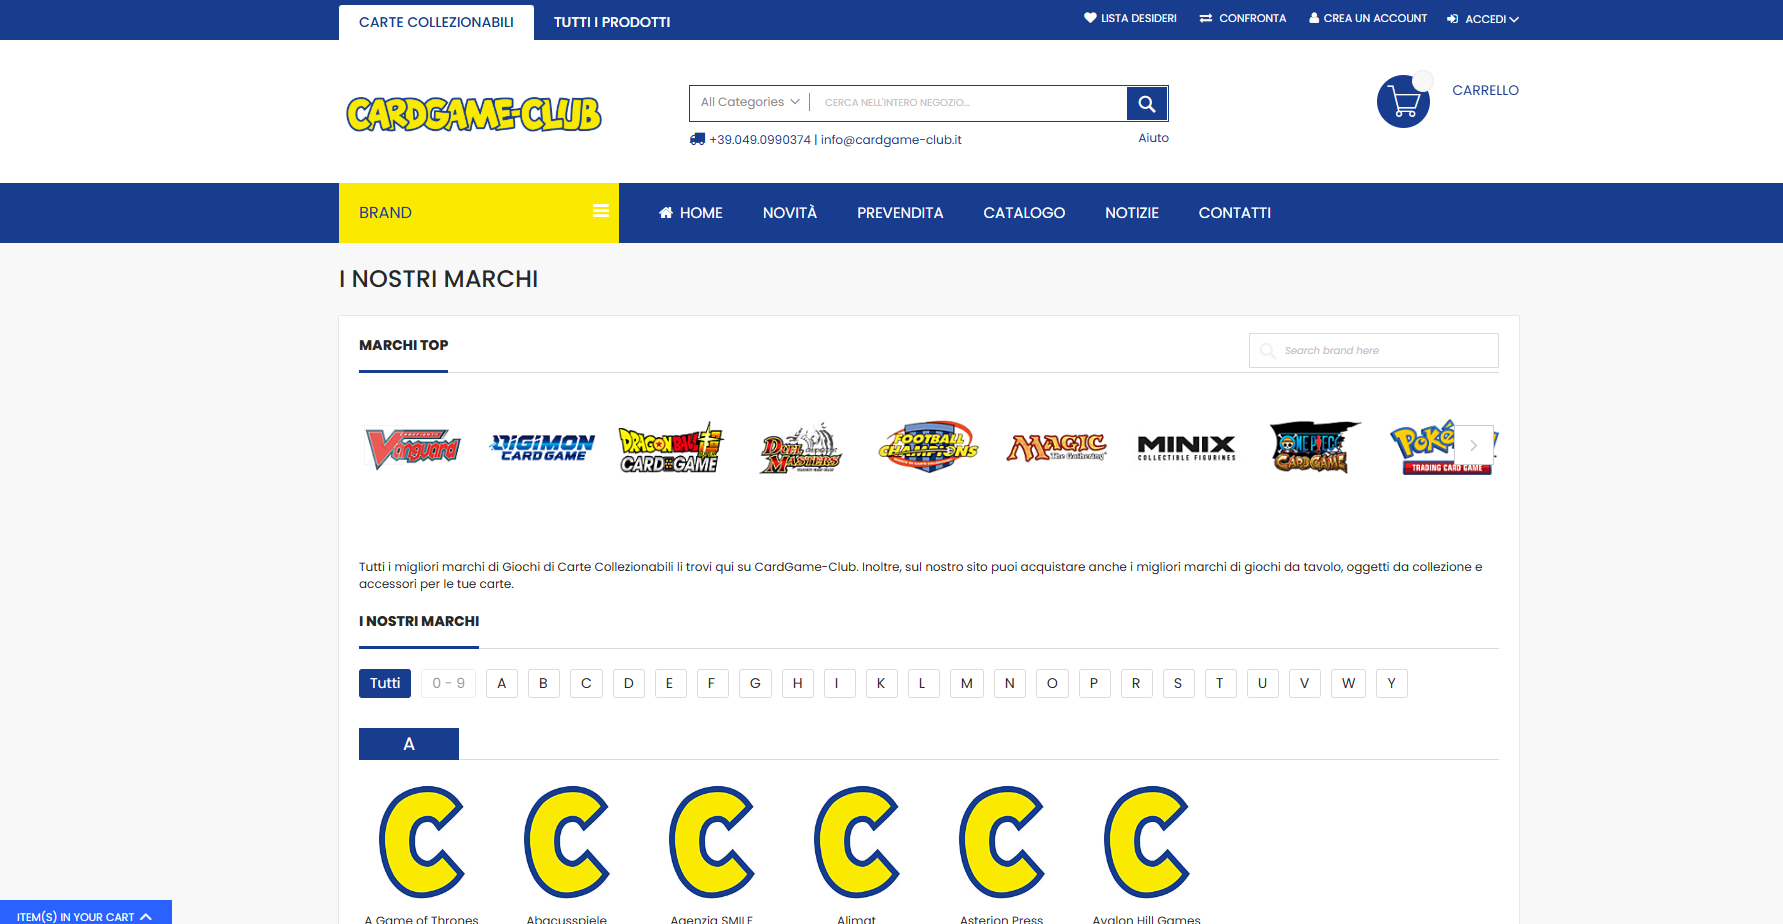
\includegraphics[width=0.8\textwidth]{cardgame.png}
    \caption{Navigazione per brand Cardgame-Club}
    \label{fig:cardgameclub}
\end{figure}

\begin{itemize}
    \item \textbf{Offerta Prodotti:} La gamma di prodotti è molto vasta, includendo numerosi TCG (dai più noti come Pokémon, Yu-Gi-Oh!, Magic, a giochi meno diffusi), sia in formato sigillato che carte singole (anche gradate o datate). Offre una selezione estesa di accessori di marchi come Ultra Pro, Dragon Shield, Ultimate Guard, oltre a giochi da tavolo e Funko Pop.
    \item \textbf{Interfaccia e Navigazione:} La navigazione si basa prevalentemente sulla selezione del marchio o del gioco. L'interfaccia appare funzionale ma potenzialmente complessa data la grande quantità di categorie e prodotti gestiti.
    \item \textbf{Funzionalità Principali:} Le funzionalità centrali sono legate alla navigazione del vasto catalogo tramite categorie e marchi, alla ricerca di prodotti specifici, al carrello acquisti e alla gestione dell'account utente. La profondità del catalogo suggerisce la possibile presenza sia di novità che di articoli fuori produzione.
\end{itemize}

% -----------------------------------------

\chapter{Funzionalità del sito}
Le funzionalità di CardHaven saranno differenziate per tipologia di utente.

\section{Funzionalità lato amministratore}
Il pannello di amministrazione (accessibile tramite autenticazione) permetterà la gestione completa del negozio:
\begin{itemize}
    \item \textbf{Gestione Catalogo Prodotti:} Inserimento, modifica, visualizzazione ed eliminazione di tutti i prodotti in vendita: carte singole, prodotti sigillati (bustine, box, mazzi precostruiti), accessori (sleeves, deck box, playmat, dadi, etc.) e gadget. Per ogni prodotto si potranno definire attributi specifici (gioco, set, rarità, lingua, immagine, descrizione, prezzo, quantità).
    \item \textbf{Gestione Categorie e Attributi:} Creazione e gestione delle categorie merceologiche (es. Magic, Pokémon, Accessori $\rightarrow$ Sleeves, Accessori $\rightarrow$ Playmat) e degli attributi per i filtri di ricerca (es. Espansione, Tipo Carta, Marca Accessorio).
    \item \textbf{Gestione Ordini:} Visualizzazione e gestione degli ordini ricevuti. Possibilità di filtrare per cliente, stato (in lavorazione, spedito, etc.), e intervallo di date. Aggiornamento dello stato dell'ordine.
    \item \textbf{Gestione Utenti:} Visualizzazione e gestione degli account degli utenti registrati.
    \item \textbf{Gestione Recensioni:} Moderazione delle recensioni inviate dagli utenti (approvazione o rifiuto/eliminazione di recensioni non conformi alle linee guida).
\end{itemize}

\section{Funzionalità lato utente registrato}
Gli utenti registrati avranno accesso a tutte le funzionalità del sito:
\begin{itemize}
    \item \textbf{Gestione Account:} Registrazione, login, logout. Modifica dei dati personali, indirizzi e password.
    \item \textbf{Navigazione e Ricerca Catalogo:} Esplorazione del catalogo per gioco, tipo di prodotto (carte, accessori, gadget), set/espansione. Ricerca testuale e applicazione di filtri avanzati. Visualizzazione dettagliata dei prodotti.
    \item \textbf{Gestione Carrello:} Aggiunta, modifica quantità, rimozione prodotti dal carrello.
    \item \textbf{Checkout:} Completamento dell'acquisto specificando indirizzo e metodo di pagamento.
    \item \textbf{Storico Ordini:} Consultazione degli ordini effettuati e del loro stato.
    \item \textbf{Scrittura Recensioni:} Possibilità di scrivere e inviare recensioni (testo e valutazione numerica, es. 1-5 stelle) per i prodotti presenti nel catalogo. Le recensioni saranno soggette a moderazione prima della pubblicazione.
    \item \textbf{Visualizzazione Recensioni:} Leggere le recensioni lasciate da altri utenti sulle pagine dei prodotti.
    \item \textbf{Wishlist/Lista Desideri:} Salvare prodotti preferiti per consultazione futura.
\end{itemize}


\section{Funzionalità lato guest}
I visitatori non autenticati potranno:
\begin{itemize}
    \item \textbf{Navigazione e Ricerca Catalogo:} Esplorare l'intero catalogo prodotti (carte, accessori, gadget) e utilizzare le funzionalità di ricerca e filtro.
    \item \textbf{Visualizzazione Recensioni:} Leggere le recensioni pubblicate dagli utenti registrati sulle pagine dei prodotti.
    \item \textbf{Gestione Carrello:} Aggiungere prodotti al carrello, modificarne la quantità e rimuoverli.
    \item \textbf{Registrazione/Login:} Accedere alle funzioni di registrazione o login per poter procedere all'acquisto o usufruire delle funzionalità riservate.
    \item \textbf{Limitazioni:} Impossibilità di finalizzare l'acquisto (verrà richiesto login/registrazione al checkout), scrivere recensioni, accedere allo storico ordini e alla gestione dell'account.
\end{itemize}

%-----------------------------------------------------------------------------------------------------
\chapter{Schema ER della base di dati}
\begin{figure}[h!]
    \centering
    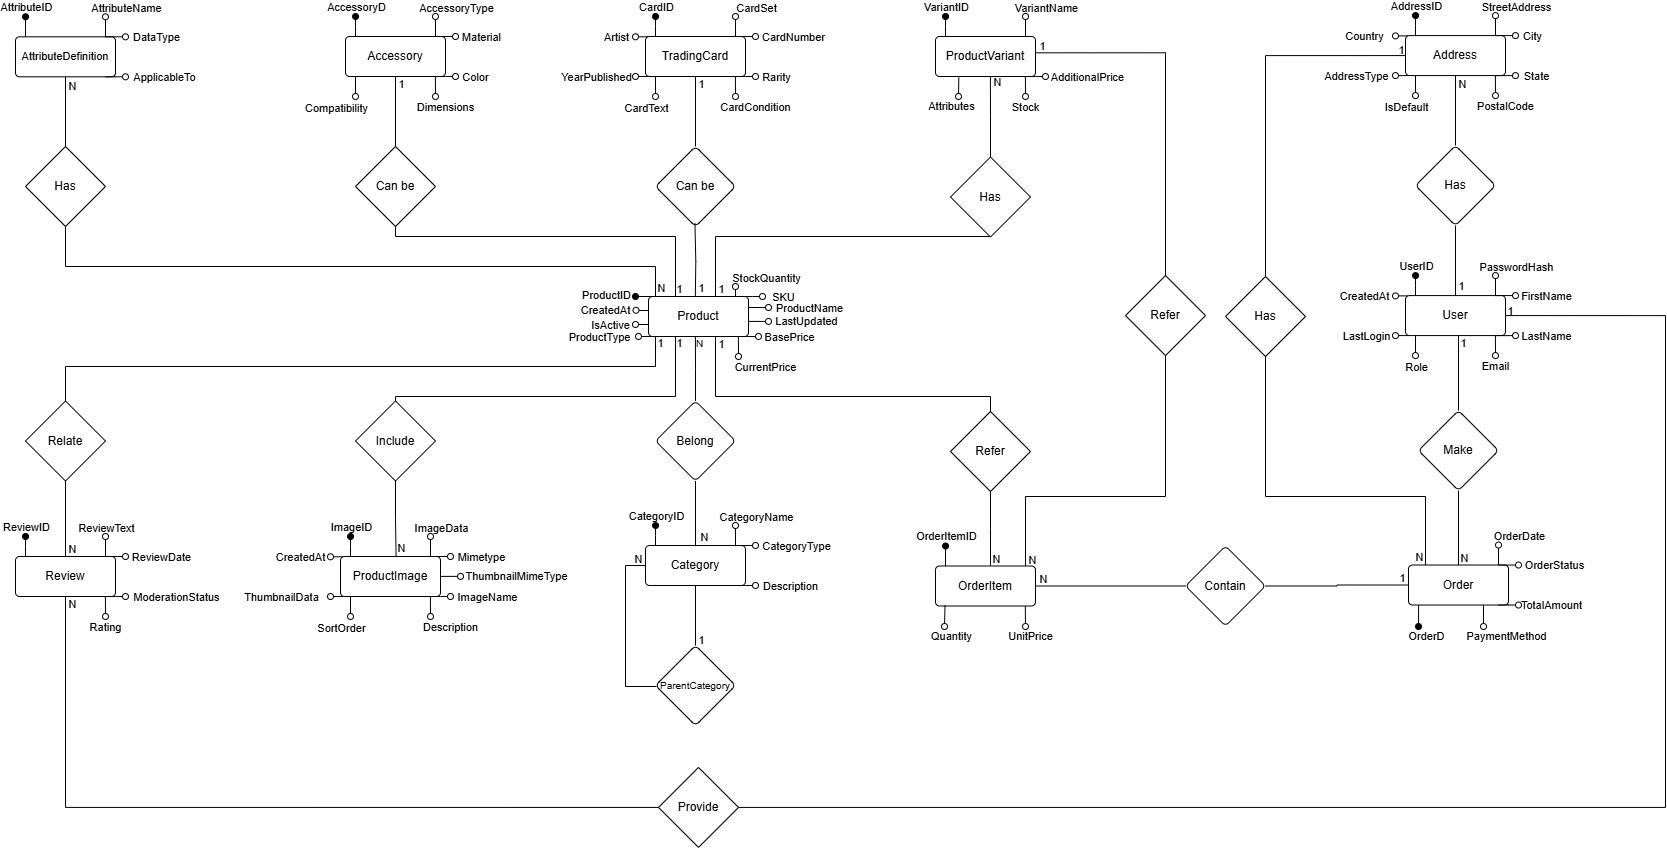
\includegraphics[width=1.1\textwidth]{cardHaven.jpg}
\end{figure}





\end{document} % Fine Documento
